\documentclass{scrartcl}
\usepackage{textcomp}
\usepackage{graphicx}
\usepackage{caption}
\usepackage{subcaption}
\usepackage[authoryear]{natbib}
\usepackage{gensymb}
\usepackage{amssymb,amsmath}
\usepackage{wrapfig}
\usepackage[toc,page]{appendix}
\usepackage{verbatim}
\usepackage{import}
\usepackage{rotating}
\usepackage{amsmath}
\usepackage{float}
\usepackage[top=0.5in, bottom=1.25in, left=1.25in, right=1.25in]{geometry}
%\usepackage[caption=false]{subfig}
\title{The Mantle Wedge: Dynamic Controls on Chemistry\\ 9 month report}
\author{Alexander Perrin}
\begin{document}

\bibliographystyle{plainnat}
\bibliography{/home/ap4909/Dropbox/PhD/ongoing_results/2015_ongoing_results/seismic,/home/ap4909/Dropbox/PhD/ongoing_results/2015_ongoing_results/geochemistry,/home/ap4909/Dropbox/PhD/ongoing_results/2015_ongoing_results/geodynamics}
\section{Southern Marianas samples}

\begin{figure}[H]
%/data/ap4909/30.10.2013-hot_cold_geochem/sample_testing/south_lesser_antilles/find_ref_h2o.py
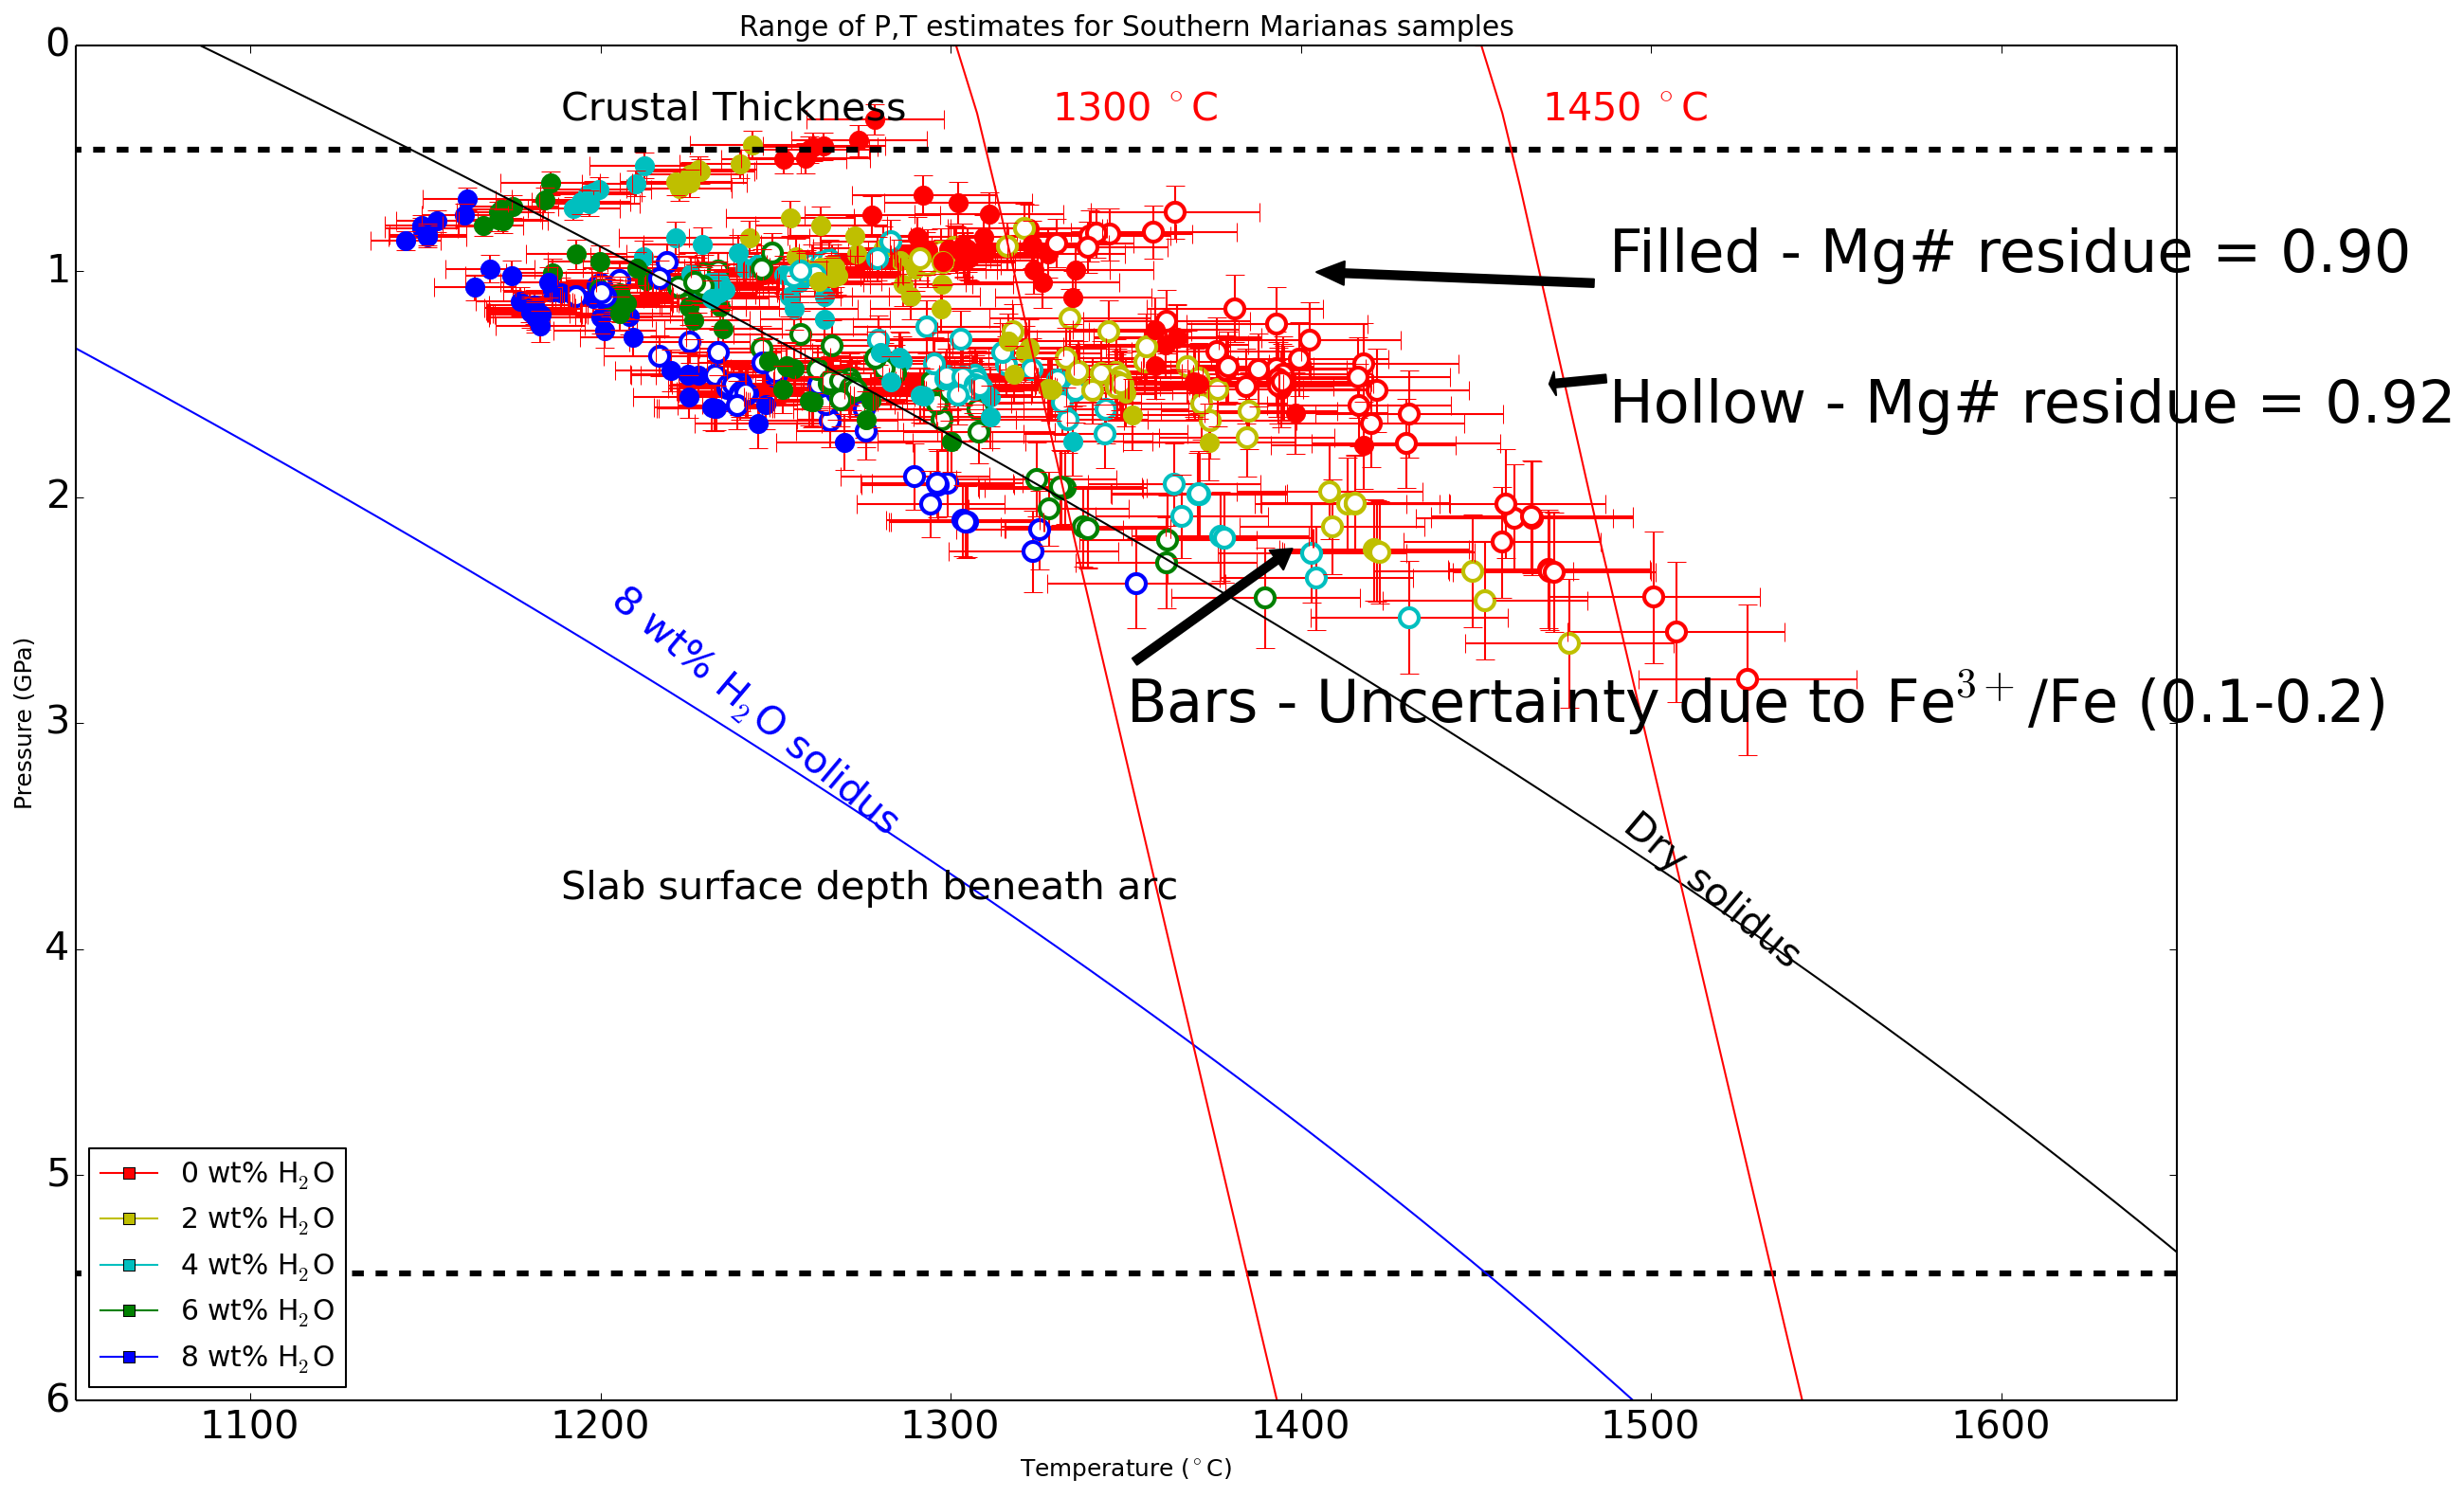
\includegraphics[width=0.9\textwidth]{/data/ap4909/30.10.2013-hot_cold_geochem/sample_testing/southern_marianas/figures/p_t_plots/h2o_evaluation_Southern_Marianas.png}
\captionsetup{singlelinecheck=off}
\caption[balals]{

}
\end{figure} 



\end{document}
